% source: https://git.fslab.de/mmklab/latex-templates/tree/master/presentation

\documentclass{beamer}

%\useoutertheme{progress}

\usepackage{etoolbox}
\newtoggle{german}

% % % % % LANGUAGE % % % %
% Make your choice here
\togglefalse{german} % English
%\toggletrue{german} % German
% % % % % \LANGUAGE % % % %

% % % Handouts % % %
%\usepackage{handoutWithNotes}
%\pgfpagesuselayout{2 on 1 with notes landscape}[a4paper,border shrink=5mm]
% % % Handouts % % %


\iftoggle{german}{
\usepackage[ngerman]{babel} % Deutsche Sprachanpassungen
\usepackage[T1]{fontenc}    % Silbentrennung bei Sonderzeichen
\usepackage[utf8]{inputenc} % Direkte Angabe von Umlauten im Dokument.Wenn Sie an einem Mac sitzen,verwenden Sie ggf. „macce“ anstatt „utf8“.
\usepackage[autostyle=true,german=quotes]{csquotes} % Anfuehrungszeichen\
}{
\usepackage[utf8]{inputenc}}

\usepackage[utf8]{inputenc}
\usepackage[T1]{fontenc}
\usepackage{textcomp}
\setbeamercovered{transparent}
\usepackage{default}
\usepackage{lmodern}
\usepackage{amsmath,amsfonts,amssymb} % Mathe
\usepackage{graphicx,wrapfig,lipsum}
\usepackage{eurosym}
\usepackage{tikz}
\usepackage{graphicx}
%\usepackage[labelformat=empty]{caption}
\usepackage{verbatim}
\usepackage{color}
\usepackage{hypernat}
\usepackage{tabularx}
\usepackage[]{units}
\usepackage{caption}
\usepackage{comment}
%\usepackage{subfigure}
\usepackage{wasysym}
\usepackage{ulem}
\usepackage[printonlyused]{acronym} 
\usepackage{tabularx}
\usepackage{appendixnumberbeamer}
\usepackage{epigraph}
\usepackage{remreset}% tiny package containing just the \@removefromreset command
\usepackage{subcaption}
\usepackage{makecell}
\usepackage{pdfpcnotes}% Usefull package for notes for presentations
\usepackage{colorbar}
%\usepackage{./progbar}
%\usepackage{./beamerouterthemeprogress}

\let\Tiny=\tiny % Reduces a few recent error on Unix systems

\usepackage[sorting=none,style=numeric-comp,backend=bibtex,firstinits=true]{biblatex} % load the package
\addbibresource{./bibliography.bib} % Add your bib file
\renewcommand*{\bibfont}{\footnotesize}

% % % % Style % % % %
% Some colours as used in other programms like openoffice
\definecolor{red}{RGB}{184,71,71}
\definecolor{green}{RGB}{51,204,102}
\definecolor{blue}{RGB}{0,100,255}
\definecolor{fhblau}{rgb}{0.3,0.2,0.5}
\definecolor{fhg}{rgb}{0.2,0.5,1}

\setbeamercolor{title}{bg=fhblau, fg=white}
\setbeamercolor{frametitle}{bg=fhblau, fg=white}
\setbeamercolor{structure}{fg=fhblau}

% MISC Styles %
\setbeamertemplate{bibliography item}[text]
\usetheme{Boadilla}
\setbeamertemplate{footline}[frame number]
\setbeamertemplate{caption}[numbered]
\setbeamersize{text margin left=0.3cm,text margin right=0.3cm}
\setbeamertemplate{navigation symbols}{}%remove navigation symbols
\makeatletter
\@removefromreset{subsection}{section}
\makeatother
\setcounter{subsection}{1}


% Here are some usefulf different fonts. Use them in every flooting enviroment with \usebeamerfont{AAA}
\setbeamerfont{AAA}{size*={16.00}{15.00}}
\setbeamerfont{aaa}{size*={12.00}{11.00}}
\setbeamerfont{bbb}{size*={11.00}{11.00}}
\setbeamerfont{ccc}{size*={10.00}{11.00}}
\setbeamerfont{ddd}{size*={9.00}{11.00}}
\setbeamerfont{eee}{size*={8.00}{11.00}}
\setbeamerfont{fff}{size*={7.75}{10.75}}
\setbeamerfont{ggg}{size*={7.50}{10.50}}
\setbeamerfont{hhh}{size*={7.25}{10.25}}
\setbeamerfont{iii}{size*={7.00}{10.00}}
\setbeamerfont{jjj}{size*={6.00}{9.00}}
\setbeamerfont{kkk}{size*={5.00}{8.00}}
\setbeamerfont{lll}{size*={4.00}{7.00}}
\setbeamerfont{mmm}{size*={3.00}{6.00}}
\setbeamerfont{nnn}{size*={2.00}{5.00}} 

% Set some beamer fonts
\setbeamerfont{title}{size=\Large,series=\bfseries,parent=structure}
\setbeamerfont{caption}{size=\footnotesize}
\setbeamertemplate{footline}[text line]{%
	\parbox{\linewidth}{\vspace*{-8pt}\hspace{1em}\insertshortauthor\hspace{8mm} Qualitative Analysis of Optical Flow for Motion Anomaly Detection \hfill\insertpagenumber/\inserttotalframenumber}}

\renewcommand*{\bibfont}{\usebeamerfont{kkk}}
\makeatletter
\newcommand\mathcircled[1]{%
  \mathpalette\@mathcircled{#1}%
}
\newcommand\@mathcircled[2]{%
  \tikz[baseline=(math.base)] \node[draw,circle,inner sep=1pt] (math) {$\m@th#1#2$};%
}
\makeatother
% A new cell type
\newcommand{\specialcell}[2][c]{%
  \begin{tabular}[#1]{@{}c@{}}#2\end{tabular}}

% This is usefull if you want to use enumerations over several frames
\newcounter{saveenumi}
\newcommand{\seti}{\setcounter{saveenumi}{\value{enumi}}}
\newcommand{\conti}{\setcounter{enumi}{\value{saveenumi}}}

% logo of my university
\titlegraphic{
\centering %
\includegraphics[height=1.5cm]{./logos/logo_hbrs.png} \hspace{2cm} % For external companies

\includegraphics[height=1.2cm]{./logos/logo_hbrs.png}}

\iffalse
\AtBeginSection[]{
  \begin{frame}[plain,noframenumbering]
      \addtocounter{framenumber}{-1}
  \vfill
  \centering
  \begin{beamercolorbox}[sep=8pt,center,shadow=true,rounded=true]{title}
    \usebeamerfont{title}\insertsectionhead\par%
  \end{beamercolorbox}
  \vfill
  \end{frame}
}
\fi

\AtBeginSection[]{
  \begin{frame}[plain]{Table of Contents}
  	\tableofcontents[currentsection, hideallsubsections]
   	%\addtocounter{framenumber}{-1}
  \end{frame}
}


% % % % % Opening % % % %
\title[]{Qualitative Analysis of Optical Flow for Motion Anomaly Detection}
\author[Pranav Megarajan]{Pranav Megarajan \\[3mm]{\usebeamerfont{eee} Supervised by:
\usebeamerfont{ccc}\\[2mm] Prof. Dr. Paul G. Pl\"{o}ger \\ [0.5mm] M. Sc. Santosh Thoduka}}
\date{\today}
%\institute[HBRS]{Hochschule Bonn-Rhein-Sieg}
\def\ThesisPubDate{\today} % Change here to the date you are going to print your thesis
\subject{Qualitative Analysis of Optical Flow for Motion Anomaly Detection}
\keywords{}


\begin{document}

% Title Frame
\begin{frame}
\pnote{Here are some nodes. They are not visible on the first slides} % Notes
\titlepage
\end{frame}

\iftoggle{german}{
%\begin{frame}{Agenda}
%\usebeamerfont{ccc}
%\tableofcontents
%\end{frame}
%}{
\begin{frame}{Table of Contents}
\usebeamerfont{ccc}
\tableofcontents
\end{frame}
}

\section{Problem}
% First Frame
\begin{frame}{Problem}
\textbf{\textcolor{fhblau}{Motion Anomaly Detection}}\\[1mm]
\begin{itemize}
\item Anomaly is a context specific term.
\item Motion Anomaly Detection: Learn the normal motion patterns and detect anomalies as non-conformities.
\item This approach is efficient only when the context and state of the system remains
constant over time. 
\item "How to detect motion anomalies as the system's context varies?
How independent can the motion anomaly detector be from the context?"


\end{itemize}


%\begin{center}
%\begin{figure}[h]
%		\centering
%	
%		\includegraphics[scale=0.35]{images/DM2.png}
%		\captionsetup{justification=centering,margin=0.2cm}
%		\caption{Classification of diagnostic algorithms \cite{VENKATASUBRAMANIAN2003293}.}
%		\label{Fig:allobjects}
%	\end{figure}
%\end{center}



\end{frame}

\section{Applications}
\begin{frame}
\frametitle{Applications}


         \begin{figure}[h]
         	\begin{subfigure}[t]{.3\textwidth}
         		%%%\vspace{0pt}
         		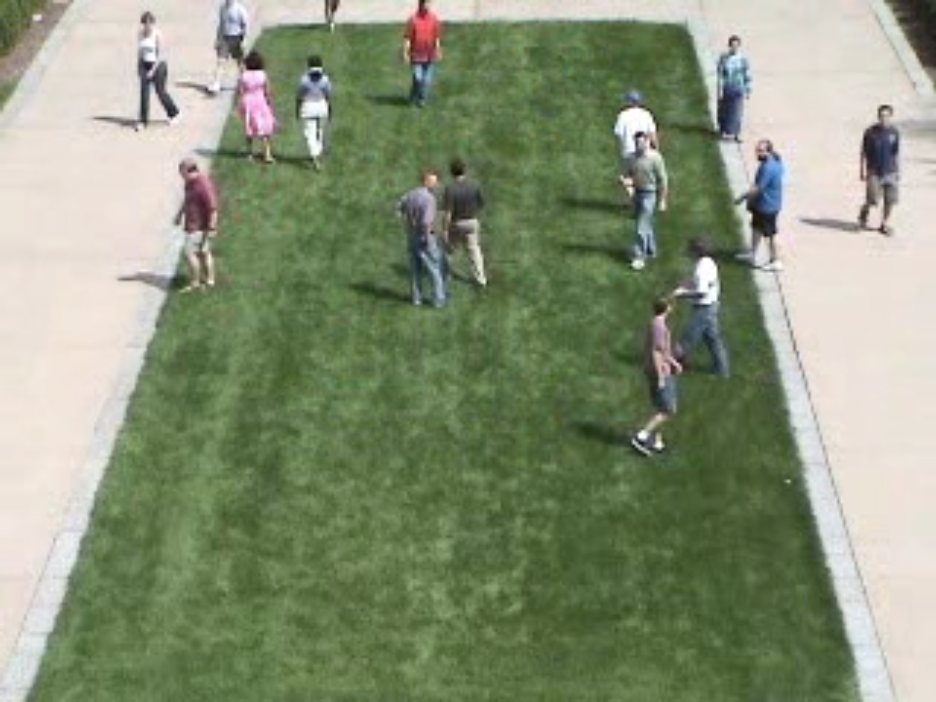
\includegraphics[width=1\linewidth]{images/umn_normal1.png}
         		\caption{Crowd Surveillance \cite{umn_crowd}}
         	\end{subfigure}\hfill%   
         	\begin{subfigure}[t]{.3\textwidth}
         		
         		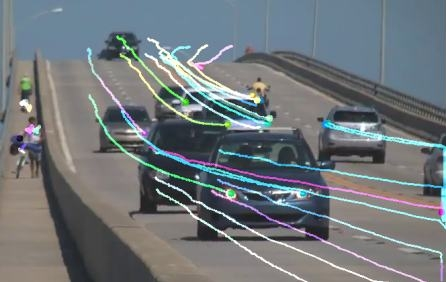
\includegraphics[height = 2.81cm,width=1\linewidth]{images/lk_flow.jpg}
         		\caption{Autonomous Cars \cite{opt_flow_opencv}}
         		
         	\end{subfigure}\hfill%
         	\begin{subfigure}[t]{.3\textwidth}
         		\centering
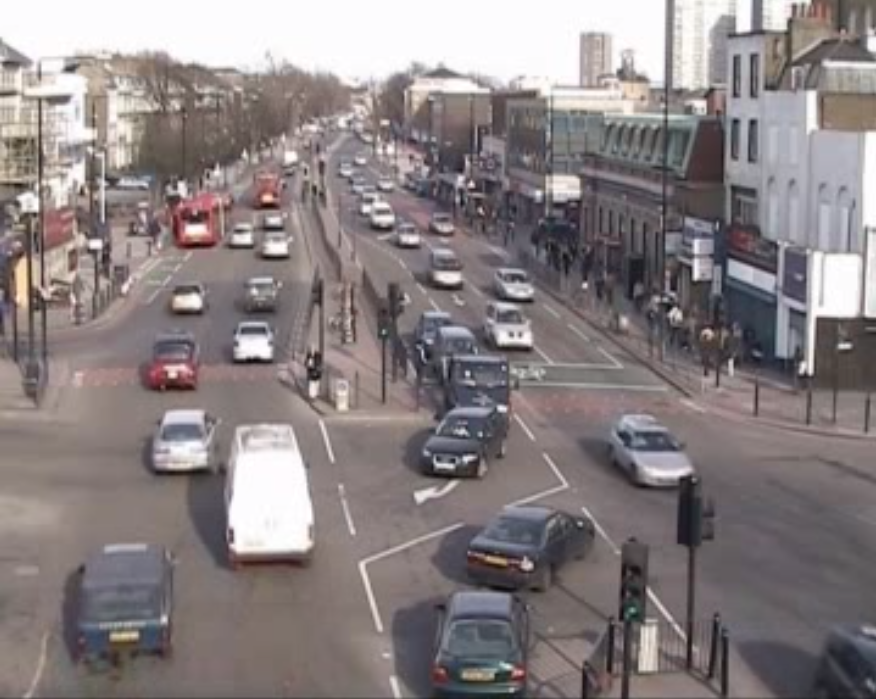
\includegraphics[width=0.98\linewidth]{images/vert_flow1.png}
         		\caption{Traffic Signals \cite{qmul_traffic}}
         		
         	\end{subfigure}
         	
         	\caption{\textbf{Application Scenarios}}
         	\label{umn_norm_ex}
         \end{figure}

\textbf{Other Applications:}  Robot Manipulation, Mobile Robots, Human-Robot Collaboration  etc.
%\textit{\usebeamerfont{eee}{Abstract Hierarchy $\rightarrow$ Structural Hierarchy $\rightarrow$ Sensor-based Fault Detection and Diagnosis (SFDD).}}
%\begin{center}
%\begin{figure}[h]
%		\centering
%	
%		\includegraphics[scale=0.32]{images/smodel.png}
%		\captionsetup{justification=centering,margin=0.2cm}
%		\caption{Structural model for SFDD \cite{2008biswas}.}
%		\label{Fig:allobjects}
%	\end{figure}
%\end{center}
%\textbf{\textcolor{fhblau}{Idea behind SFDD:}}\\[0.6mm]
%Any fault occurring in higher level system/subsystem reflects in the behaviour of its lower level elements.

\end{frame}



\section{Related Work}

\begin{frame}{Automated Crowd Surveillance}
     \begin{figure}[h]
     	\centering
     	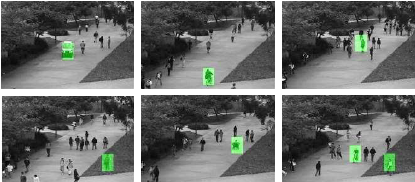
\includegraphics[scale= 0.5]{images/anom_green.png} 
     	\caption{Automated Crowd Surveillance. The green part indicates the anomalies in the crowd. \cite{ucsd_anom}}
     \end{figure}

\begin{itemize}
\item Optical Flow is used to describe the movement within the frame.
\item Several Learning methods are used to model the normal motion over the given dataset.
\end{itemize}

\end{frame}


\begin{frame}{Robot Manipulation}

\begin{figure}[]
	\centering     
	
	
	\begin{subfigure}[b]{0.5\textwidth}
		
		
			\centering
			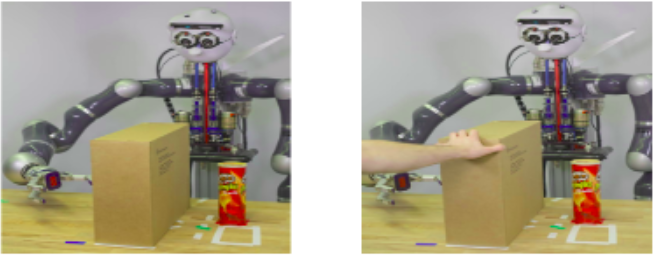
\includegraphics[width= 0.75\linewidth, height = 1.6cm]{images/hand_manip.png}
			\captionof{figure}{Hand movement causes an anomaly.}
			
	
	\end{subfigure}
	
	
	\begin{subfigure}[b]{0.5\textwidth}
		
			\centering
			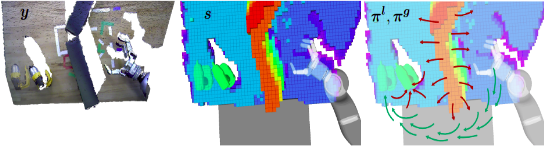
\includegraphics[width= 0.85\linewidth, height = 1.6cm]{images/second_2.png}
			\captionof{figure}{Optical Flow heat map. }
			
		
	
	\end{subfigure}
	
	
	
	\caption{Motion Anomalies in Manipulation Task \cite{hand_manip_anom}   }\label{qmul_normal_pic} 
\setlength{\belowcaptionskip}{-20pt}	
\end{figure}


\begin{itemize}
\item Optical Flow values are clustered to detect the outlier flow values.
\item Works with a moving camera or frame.
\end{itemize}

\end{frame}


\begin{frame}{Insufficiency}
\begin{itemize}
\item \textbf{Automated Crowd Surveillance: }
\begin{itemize}
\item Motion Anomalies are learnt from dataset, so as the context changes, we should relearn.
\item Learning only done with data from Fixed Frame or Camera.
\end{itemize}

\item \textbf{Robot Manipulation:}
\begin{itemize}
\item Does not work with change in context.
\end{itemize} 

\end{itemize}

Can we utilize optical flow information to detect motion anomalies from a ‘Moving
Frame/ Camera’ and can it be generalized in order to avoid ‘learning’ wherever
possible ?

\end{frame}




\section{Approach}

\begin{frame}{Optical Flow field as Vector field}
\begin{itemize}
\item Optical Flow fields are analysed using techniques used for \textbf{vector field} or \textbf{orientation field} classification.
\end{itemize}

\begin{figure}[h]
            	\centering
            	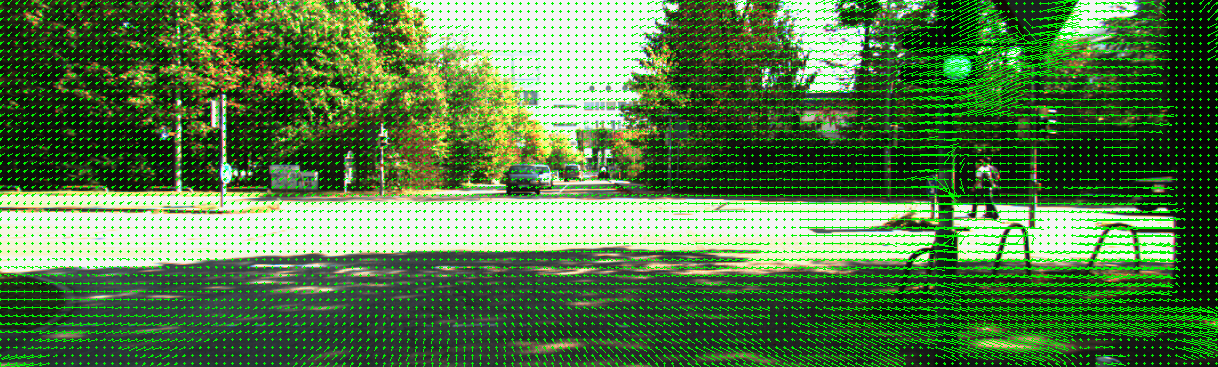
\includegraphics[width =0.5\linewidth]{images/kitti_noisy_2.png} 
            	\caption{Optical flow field superimposed on the image \cite{kitti_data}.}
            \end{figure}
       
       
       
%         \begin{figure}[h!]
%         	\centering
%         	\begin{minipage}{.3\textwidth}
%         		\centering
%         		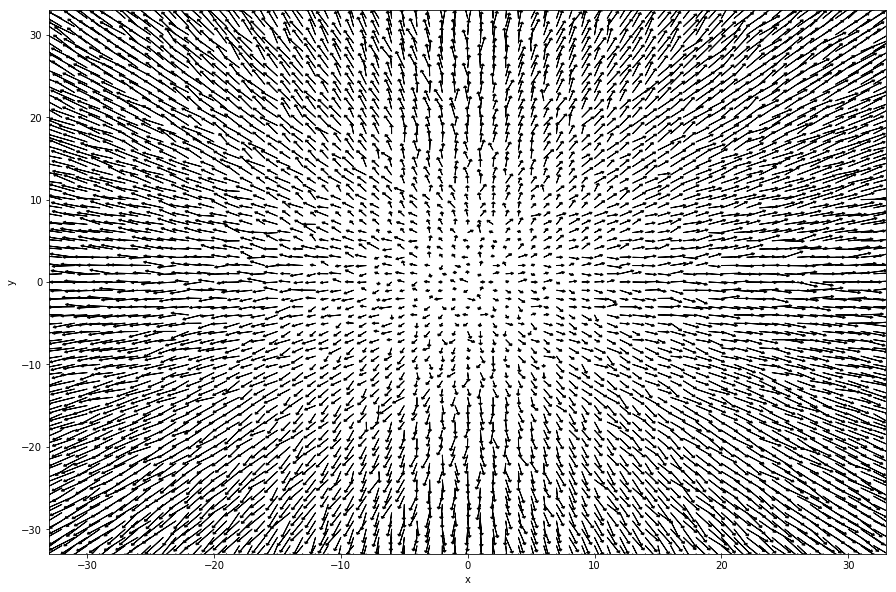
\includegraphics[width= 0.8\linewidth]{images/noisy_phase.png}
%         		\captionof{figure}{Typical noisy optical flow field}
%         		\label{noisy}
%         	\end{minipage}%
%         	\begin{minipage}{.3\textwidth}
%         		\centering
%         		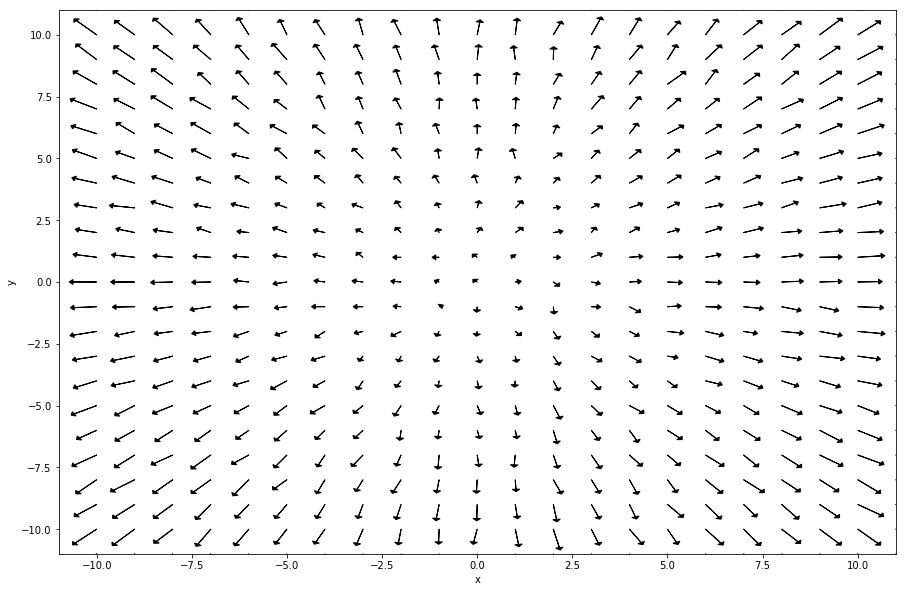
\includegraphics[width=.8\linewidth]{images/noiseless_phase.png}
%         		%\vspace*{0.5cm}
%         		\captionof{figure}{Smoothened optical flow field}
%         		\label{noiseless}
%         	\end{minipage}
%         \end{figure}
%




\begin{figure}[h]
         	\begin{subfigure}[t]{.5\textwidth}
         	\centering
         		%%%\vspace{0pt}
         		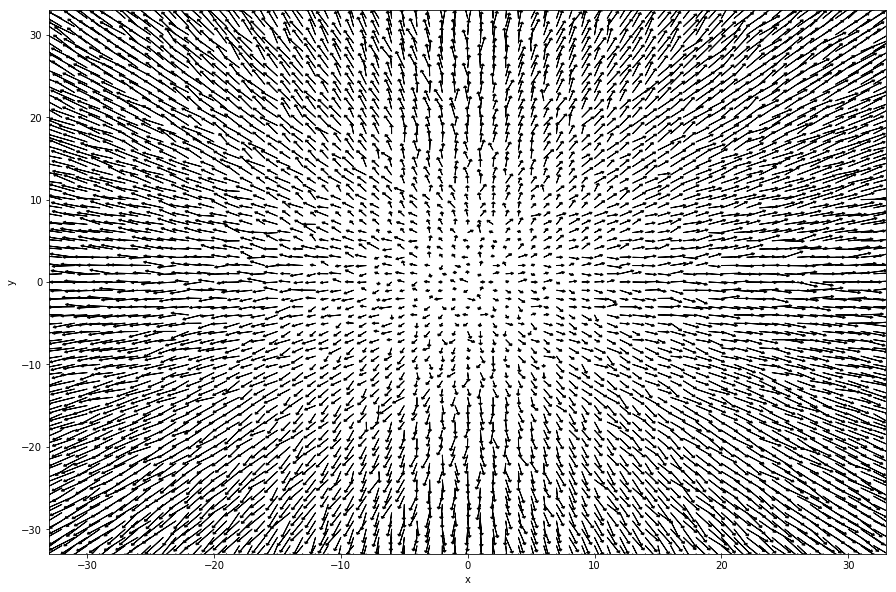
\includegraphics[height=2cm,width=0.7\linewidth]{images/noisy_phase.png}
         		\caption{Noisy flow field }
         	\end{subfigure}\hfill%   
         	\begin{subfigure}[t]{.5\textwidth}
         	\centering
         		
         		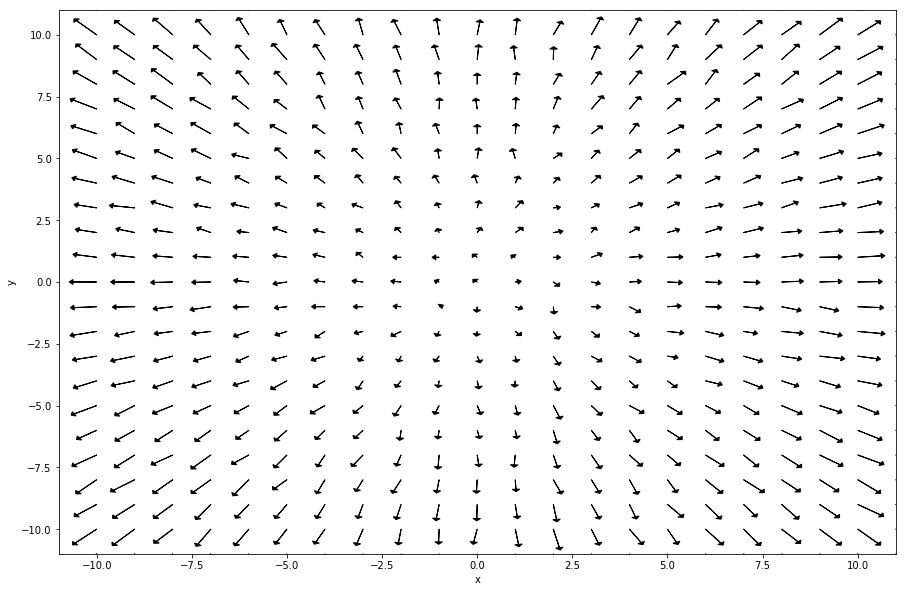
\includegraphics[height =2cm,width=0.7\linewidth]{images/noiseless_phase.png}
         		\caption{Smoothened flow field }
         		
         	\end{subfigure}

         	
         	\caption{Dominant orientations are obtained from (a) to form (b).}
         	\label{umn_norm_ex}
         \end{figure}




%If the past values of time series Y can provide better
%prediction of another time series X than past values of X alone, then, Y\textbf{ Granger causes} X.
%\\[2mm]
%
%Equations using vector autoregression model,
%
%     \begin{equation} \label{1}
% X(t) = a_0 + a_1{x_{t-1}}.....+a_p{x_{t-p}}+\epsilon_{t1} \textrm{\textcolor{fhg}{\usebeamerfont{ggg}{ \hspace{1mm}(restricted)}}}
% \end{equation}
%\raggedbottom
% \begin{equation}\label{2}
% X(t) = a_0 + a_1{x_{t-1}}.....+a_p{x_{t-p}} +b_1{y_{t-1}}.....+b_p{y_{t-p}} +\epsilon_{t2}\textrm{\textcolor{fhg}{\usebeamerfont{ggg}{ \hspace{1mm}(unrestricted)}}}
%  \vspace{3mm}
% \end{equation}
%\usebeamerfont{eee}{
% $a_i$ and $b_i$  ($i=1,2..p$) $\Rightarrow$ time-invariants.\\
% $t$ ($t=1,2,...T$) $\Rightarrow$ time .\\ 
% $\alpha_0$  $\Rightarrow$ vector of intercepts.\\
% $t-p$ $\Rightarrow$ $pth$ lag of the variable.\\
%
% $\epsilon_{ti}$ $\Rightarrow$ error terms with mean zero.
% }
% 
%      \begin{center}   	
%     	$H_0$ : $b_i = 0$ for i in $[1,p]$  \hspace{0.2cm}  (null hypothesis)\\
%     	$H_1$ : $b_i \neq 0$ for at least 1 of i for i in $[1,p]$  \hspace{0.2cm} (alternate hypothesis)
%    	
%     \end{center}

\end{frame}


\begin{frame}{Qualitative Analysis of Optical Flow}
\begin{minipage}{0.3\textwidth}
\begin{figure}
\label{wrap-fig:1}
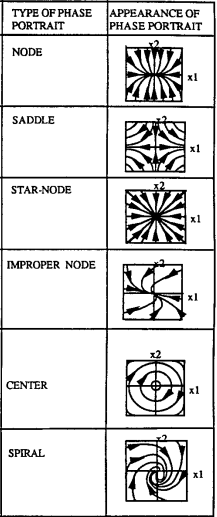
\includegraphics[width=2.5cm]{images/ph_classification_2.png}
\caption{Types of phase portraits \cite{phase_port_paper}}
\end{figure}
\end{minipage}\hfill%
\begin{minipage}{0.68\textwidth}
\begin{itemize}
\item Classification of Optical Flow field into one of the phase portraits.
\item Possible classifications are shown in Figure 6.
\item The \textbf{Characteristic equation} of the flow fields is given by:
       	\begin{equation}
       		\dot{X} = A\bar{x} + B
       	\end{equation} 
       	
       	 \begin{equation}
    \begin{bmatrix}
  \dot{x} \\
  \dot{y}
  \end{bmatrix} =  \begin{bmatrix}
  a &b\\
  c &d
  \end{bmatrix} \begin{bmatrix}
  x \\
  y
  \end{bmatrix} + \begin{bmatrix}
  e \\
  f
  \end{bmatrix}
  \end{equation}
  
  \item \textbf{Critical Point(c)}/ Fixed Point: Point of zero flow or origin.
         	\begin{equation}
       		\dot{X(c)} = 0
       	\end{equation} 

\end{itemize}
\end{minipage}


\end{frame}

\begin{frame}{Classifying Optical Flow}
\begin{figure}[]
     	\centering     
     	
     	

     	
     	
     	\begin{subfigure}[b]{0.8\textwidth}
     		\begin{minipage}{.3\textwidth}
     			\centering
     			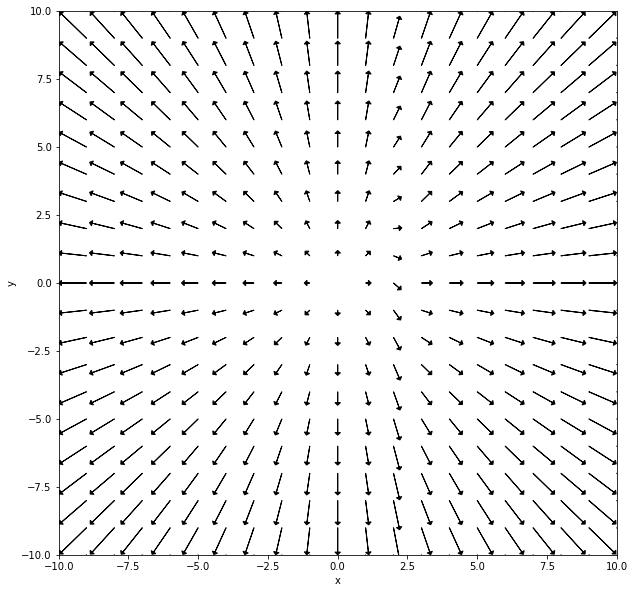
\includegraphics[width= 0.8\linewidth]{images/star_phase.png}
     			\captionof{figure}{Star Phase}
     			
     		\end{minipage}%
     		\begin{minipage}{.3\textwidth}
     			\centering
     			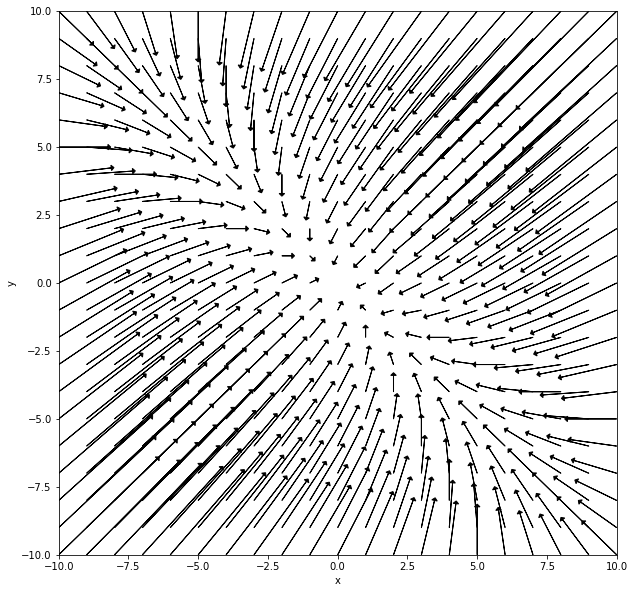
\includegraphics[width=.8\linewidth]{images/nodal_phase.png}
     			%\vspace*{0.5cm}
     			\captionof{figure}{Nodal Phase}
     			
     		\end{minipage}%
                 \begin{minipage}{.3\textwidth}
     			\centering
     			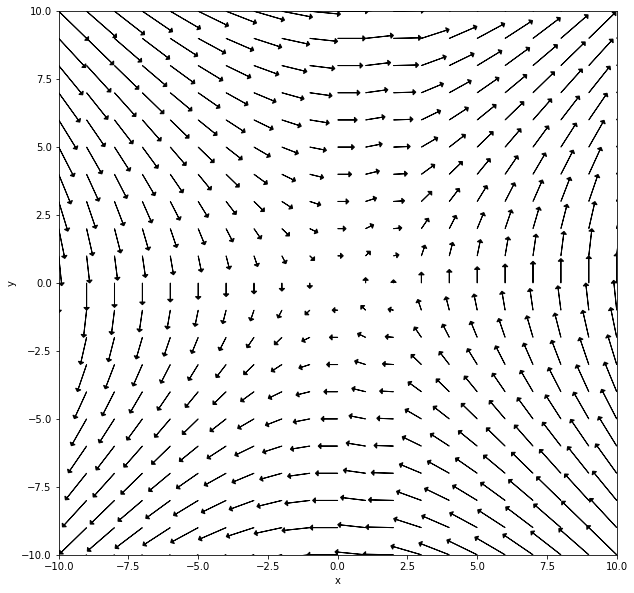
\includegraphics[width=.8\linewidth]{images/saddle_phase.png}
     			%\vspace*{0.5cm}
     			\captionof{figure}{Saddle Phase}
     			
     		\end{minipage}
     	\end{subfigure}
     	

     	\begin{subfigure}[b]{0.8\textwidth}
     		
     		\begin{minipage}{.3\textwidth}
     			\centering
     			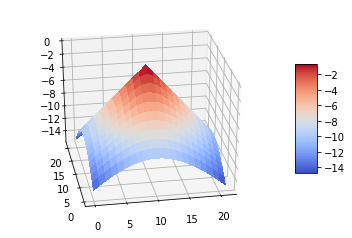
\includegraphics[width= 0.98\linewidth]{images/star.png}
     			\captionof{figure}{Equal/Same Signs }
     			
     		\end{minipage}%
     		\begin{minipage}{.3\textwidth}
     			\centering
     			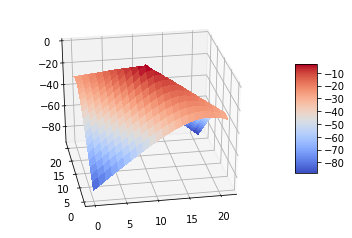
\includegraphics[width=.98\linewidth]{images/node.png}
     			%\vspace*{0.5cm}
     			\captionof{figure}{Distinct/Same Signs}
     			
     		\end{minipage}%
               \begin{minipage}{.3\textwidth}
     			\centering
     			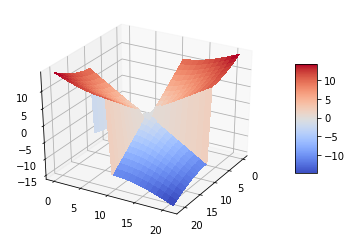
\includegraphics[width=.98\linewidth]{images/saddle.png}
     			%\vspace*{0.5cm}
     			\captionof{figure}{Distinct/ \\Different Signs}
     			
     		\end{minipage}
     	\end{subfigure}
     	
     	
     	

     	\caption{Classifications by \textbf{Eigen values} }\label{failure_1} 
     	
     \end{figure}
     
     
     \end{frame}

\begin{frame}{Classifying Optical Flow}




            \begin{figure}[h]
            	\centering
            	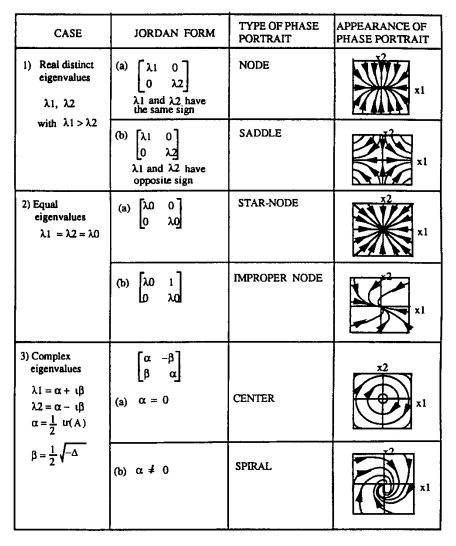
\includegraphics[width =  0.4\linewidth]{images/ph_classification_1.png} 
            	\caption{Overall classification of phase portraits based on eigenvalues and Jordan canonical forms. \cite{phase_port_paper}}
            	\label{phase_port_class}
            \end{figure}

\end{frame}


\begin{frame}{Implementation }
\textbf{Problems Faced:}
\begin{itemize}
\item Non-Linear Optimization Problem
\begin{itemize}
\item Levenberg-Marquardt - Non-Linear least Squares.
\end{itemize}
\item Time taken - Approx. 5 min/frame.
\begin{itemize}
\item Image Size = 1224x370, Window Size = 11x11.
\end{itemize}
\end{itemize}

\textbf{Solution:}
\begin{itemize}
\item \textbf{CMA-ES}(Covariance Matrix Adaptation - Evolution Strategy.)
\begin{itemize}
\item Reduced computation time to 1/4th(approx. 1.25 min/frame).
\end{itemize}
\item Devised and implemented a \textbf{linear algorithm}.
\end{itemize}
\end{frame}


\begin{frame}{Linear Algorithm}
\begin{itemize}
\item Non-linear optimization problem involved when approximating to the characteristic equation using a non-linear objective function. 
\begin{itemize}
\item \textbf{Characteristic Equation:}        	\begin{equation}
       		\dot{X} = A\bar{x} + B
       	\end{equation}
\item \textbf{Affine Transformation = Linear Transformation + Translation}
\end{itemize}
\item Non-Linear optimization problem can be avoided when the above system is approximated to:
\begin{itemize}
\item \textbf{Linear Transformation:} 
\begin{equation}
       		\dot{X} = A\bar{x}
       	\end{equation}
\end{itemize}
\item When can B be considered as a zero vector?
\begin{equation}
       		 B = 0
       	\end{equation}
\end{itemize}
\end{frame}

\begin{frame}{Linear Algorithm}
\begin{itemize}
\item B= 0 when critical point(c) and origin of co-ordinate system are same(i.e. no translation).

\begin{figure}[h]
	\centering     
	
	
	\begin{subfigure}[b]{0.4\textwidth}
		
		\begin{minipage}{.5\textwidth}
			\centering
			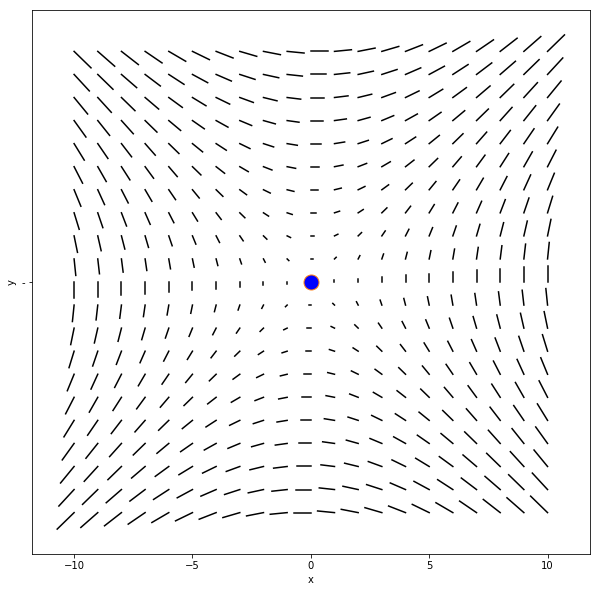
\includegraphics[width= 0.8\linewidth]{images/crit_adj2.png}
			\captionof{figure}{}
			
		\end{minipage}%
		\begin{minipage}{.5\textwidth}
			\centering
			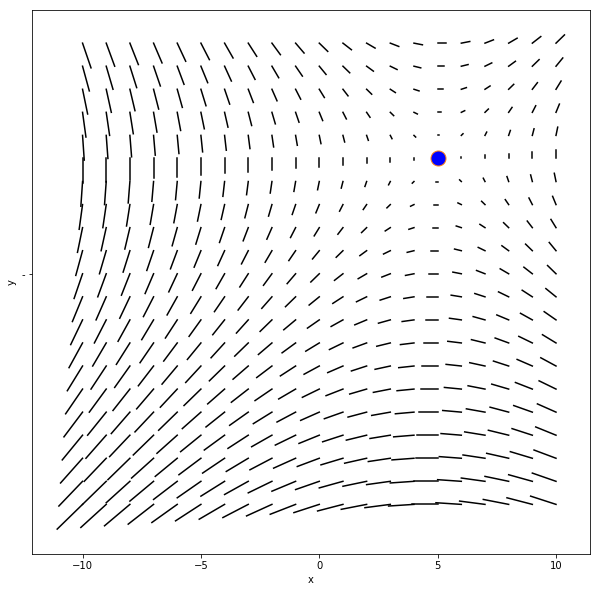
\includegraphics[width=.8\linewidth]{images/crit_adj1.png}
			%\vspace*{0.5cm}
			\captionof{figure}{}
			
		\end{minipage}
	\end{subfigure}
	
	
	\begin{subfigure}[b]{0.4\textwidth}
		\begin{minipage}{.5\textwidth}
			\centering
			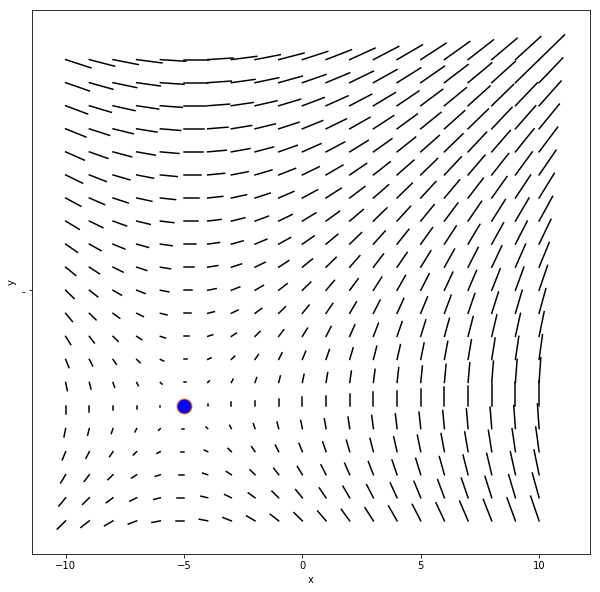
\includegraphics[width= 0.8\linewidth]{images/crit_adj3.png}
			\captionof{figure}{}
			
		\end{minipage}%
		\begin{minipage}{.5\textwidth}
			\centering
			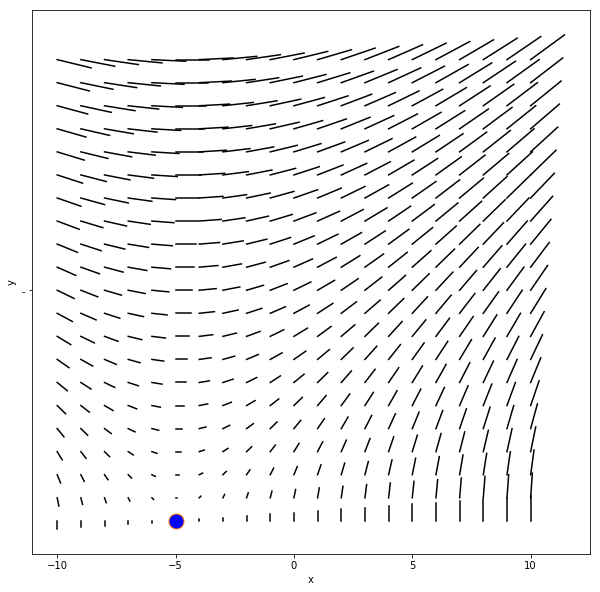
\includegraphics[width=.8\linewidth]{images/crit_adj4.png}
			%\vspace*{0.5cm}
			\captionof{figure}{}
			
		\end{minipage}
	\end{subfigure}
	
	
	
	\caption{\textbf{Effect of Translation Matrix:} The flow fields above have been created with the same linear transformation part(A) but varying B, the translation part. }\label{crit_adjust} 
	
\end{figure}        

\end{itemize}

\end{frame}

\begin{frame}{Linear Algorithm}
\begin{itemize}
\item Find the \textbf{critical point} and \textbf{shift co-ordinate system} to match with origin.
\item \textbf{Critical Point Detection:} Cluster points with similar orientation and fit lines.

\end{itemize}
 \begin{figure}[h]
 \centering
       	\begin{subfigure}[t]{.3\textwidth}
       	\centering
       		%%%\vspace{0pt}
       		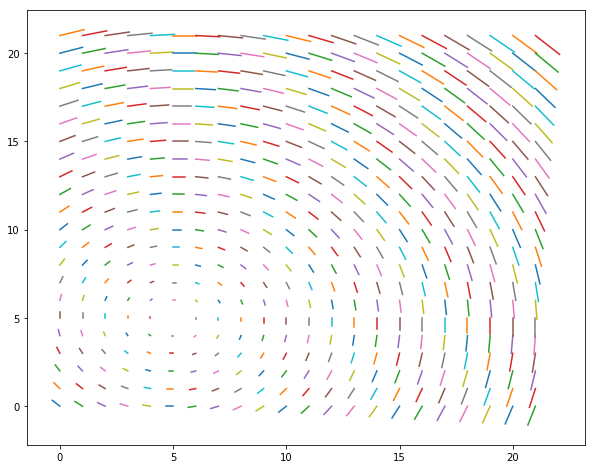
\includegraphics[width=0.6\linewidth]{images/cluster_2.png}
       		\caption{Orientation Field}
       	\end{subfigure}\hfill%   
       	\begin{subfigure}[t]{.3\textwidth}
       	\centering
       		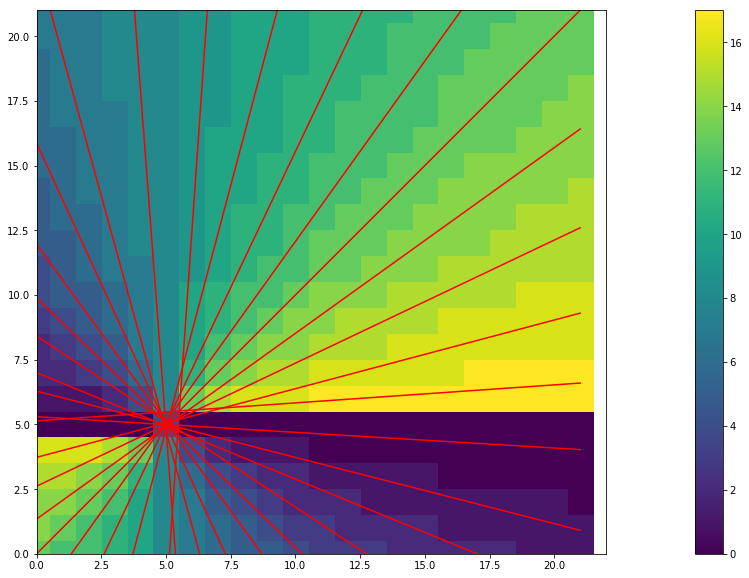
\includegraphics[width=0.6\linewidth]{images/line_clr2.png}
       		\caption{Fitted Lines}
       		
       	\end{subfigure}\hfill%
       	\begin{subfigure}[t]{.3\textwidth}
       		\centering
       		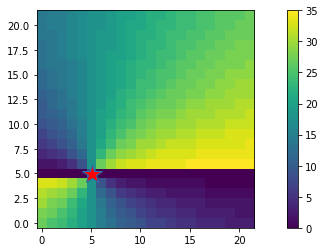
\includegraphics[width=0.6\linewidth]{images/crit_estp1_loc.png}
       		\caption{Critical point}
       	
       	\end{subfigure}
       	
       	\caption{Critical point estimation process can be seen above. Given the orientation field, the data is clustered, lines fitted and the critical point is estimated.}
       	\label{crit_steps}
       \end{figure}
    
\end{frame}

\begin{frame}{Motion Anomaly Detection}
Characteristics of the system equation:
\begin{itemize}
\item Type of \textbf{Phase portrait}
\item \textbf{Critical Point} - Point of zero flow
\item \textbf{Fit} - Closeness or similarity measure between two orientation fields.
\end{itemize}

Motion Anomalies can be detected by analysing all these characteristics !

\end{frame}
\begin{frame}{Detection by Type}
\begin{itemize}
\item  Example: Traffic Signals - Detecting Illegal Crossings and U-turns.
\end{itemize} 
\begin{figure}[h]
            	\centering
            	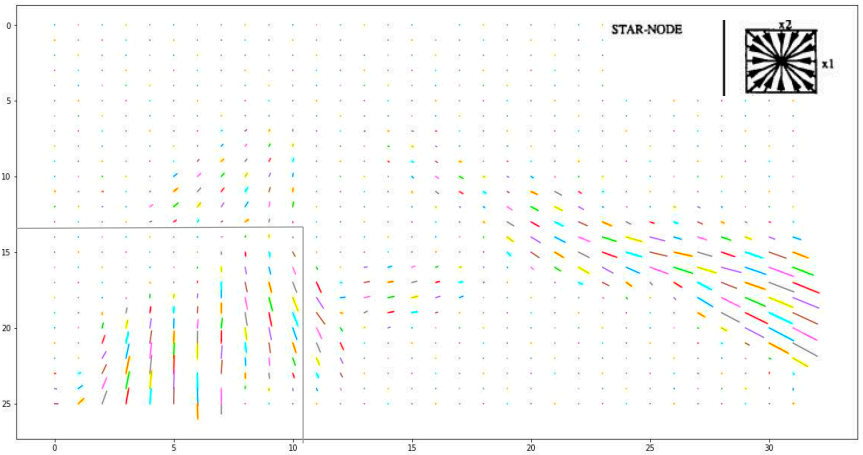
\includegraphics[width =0.65\linewidth]{images/star_pdf1.png} 
            	\caption{Orientation field obtained from the QMUL traffic signal dataset.}
            \end{figure}
\end{frame}



\begin{frame}{Detection by Type}
\begin{itemize}
\item  Example: Traffic Signals - Detecting Illegal Crossings and U-turns.
\end{itemize} 
\begin{figure}[h]
            	\centering
            	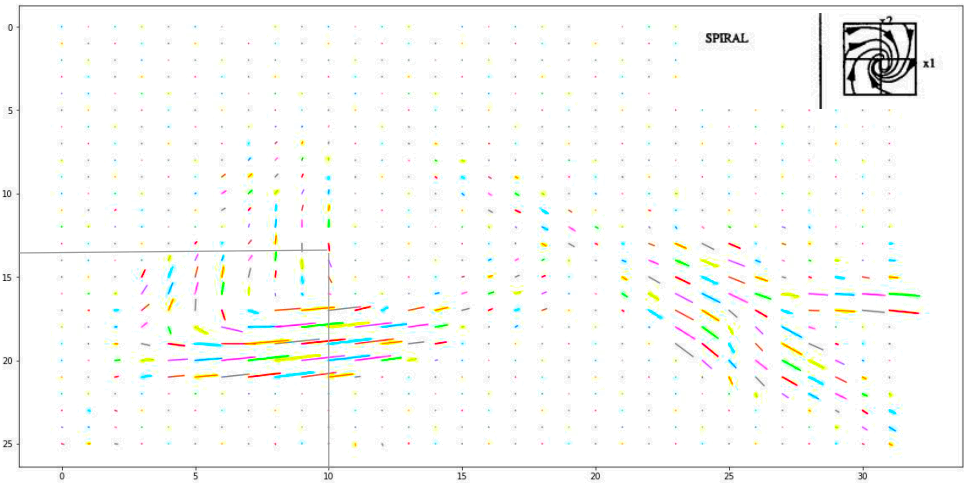
\includegraphics[width =0.65\linewidth]{images/spiral_pdf1.png} 
            	\caption{A spiral phase portrait is associated to illegal activities.}
            \end{figure}
\end{frame}


\begin{frame}{Detection by Critical Point}
\begin{itemize}
\item Example: Mobile robots/Autonomous cars - Detecting sudden turns. 
\end{itemize}
\begin{figure}[h]
            	\centering
            	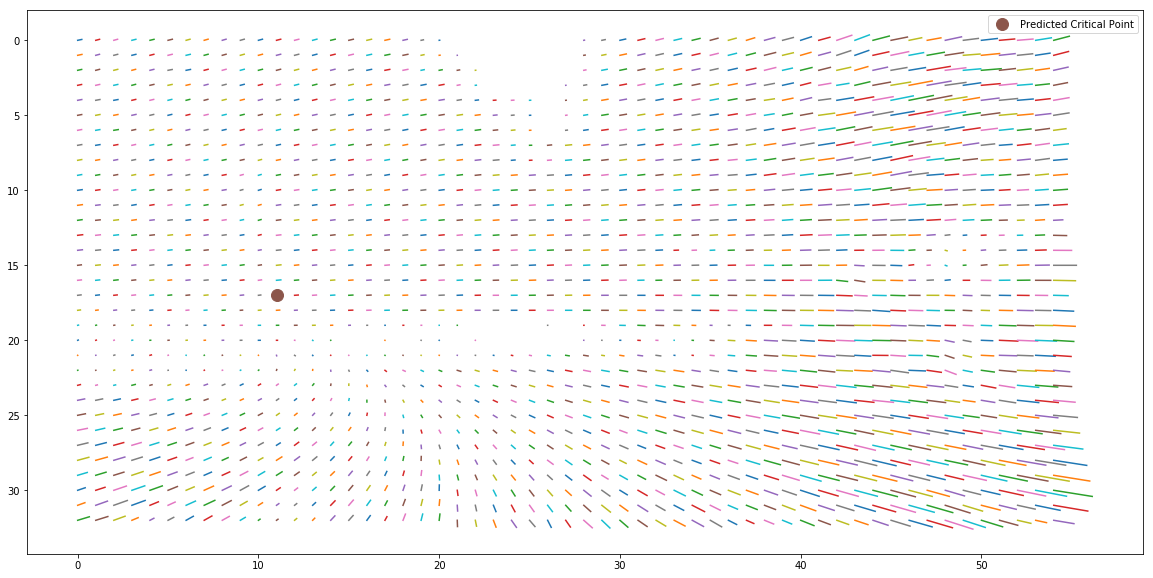
\includegraphics[width =0.65\linewidth]{images/1117critturn1.png} 
            	\caption{Critical point seen to the left extreme.}
            \end{figure}
\end{frame}


\begin{frame}{Detection by Critical Point}
\begin{itemize}
\item Example: Mobile robots/Autonomous cars - Detecting sudden turns. 
\end{itemize}
\begin{figure}[h]
            	\centering
            	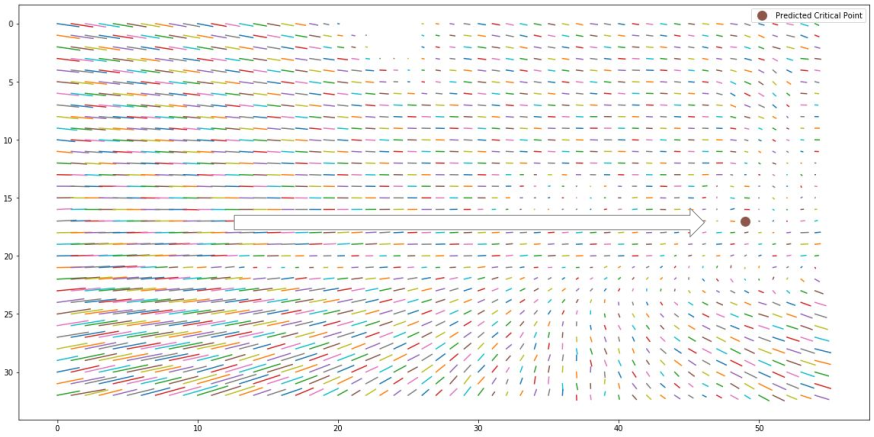
\includegraphics[width =0.65\linewidth]{images/49_17_critturn2.png} 
            	\caption{Drastic shift in critical point.}
            \end{figure}
\end{frame}


\begin{frame}{Detection by Fit}
\begin{figure}[h!]
	\begin{subfigure}[t]{1\textwidth}
		%%%\vspace{0pt}
		
		\centering
		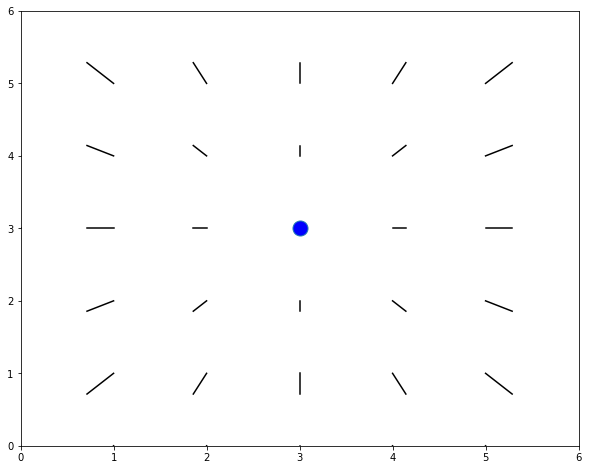
\includegraphics[width=0.25\linewidth]{images/fit_match1.png}
		
		\caption{Mapped phase portrait}
	\end{subfigure}   
	\begin{subfigure}[t]{.25\textwidth}
		
		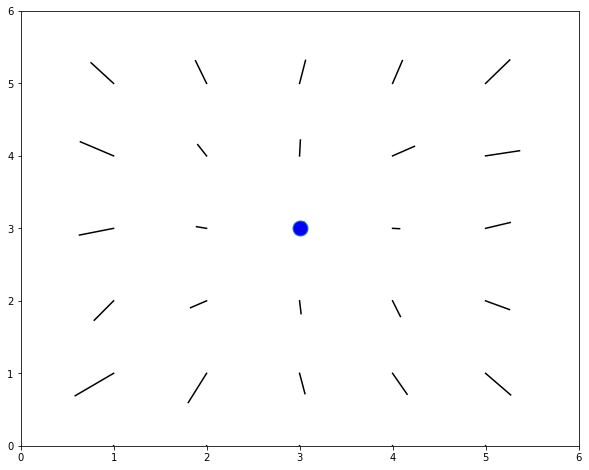
\includegraphics[width=\linewidth]{images/fit_match_a.png}
		\caption{Field (t-1) }
		
	\end{subfigure}\hfill%
	\begin{subfigure}[t]{.25\textwidth}
		\centering
		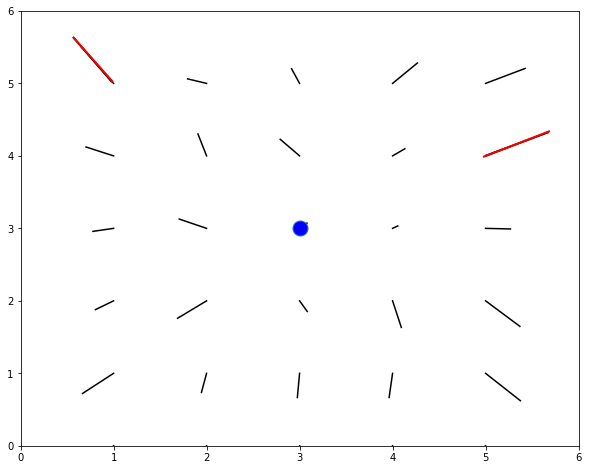
\includegraphics[width=1\linewidth]{images/fit_match_b.png}
		\caption{Field (t)}
		
	\end{subfigure}
	
	\caption{\textbf{Variance by Fit:} Two orientation fields share the same phase portrait and critical point but the fit varies. Fit is a measure of closeness or similarity.  }
	\label{fit_vary}
\end{figure}

\end{frame}




\section{Experiments and Results}


\begin{frame}{Experiment - Dataset}
\begin{itemize}
\item The dataset that was chosen for the experiment was the \textbf{UMN crowd activity}\cite{umn_crowd} dataset by the University of Minnesota.


\begin{figure}[h]
         	\begin{subfigure}[t]{.3\textwidth}
         		%%%\vspace{0pt}
         		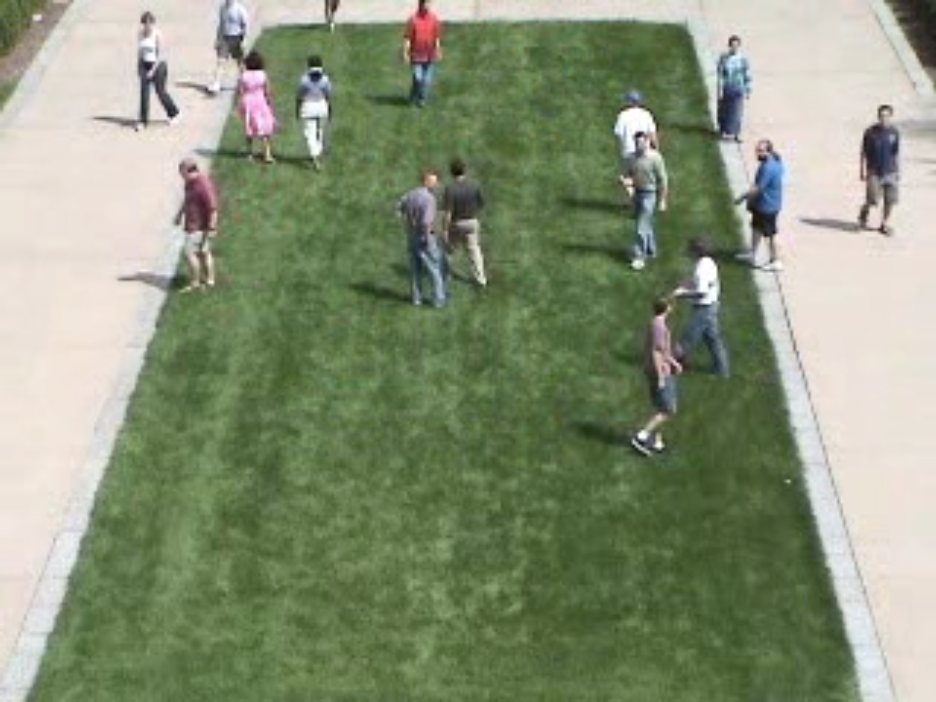
\includegraphics[width=0.8\linewidth]{images/umn_normal1.png}
         		\caption{Gardens}
         	\end{subfigure}\hfill%   
         	\begin{subfigure}[t]{.3\textwidth}
         		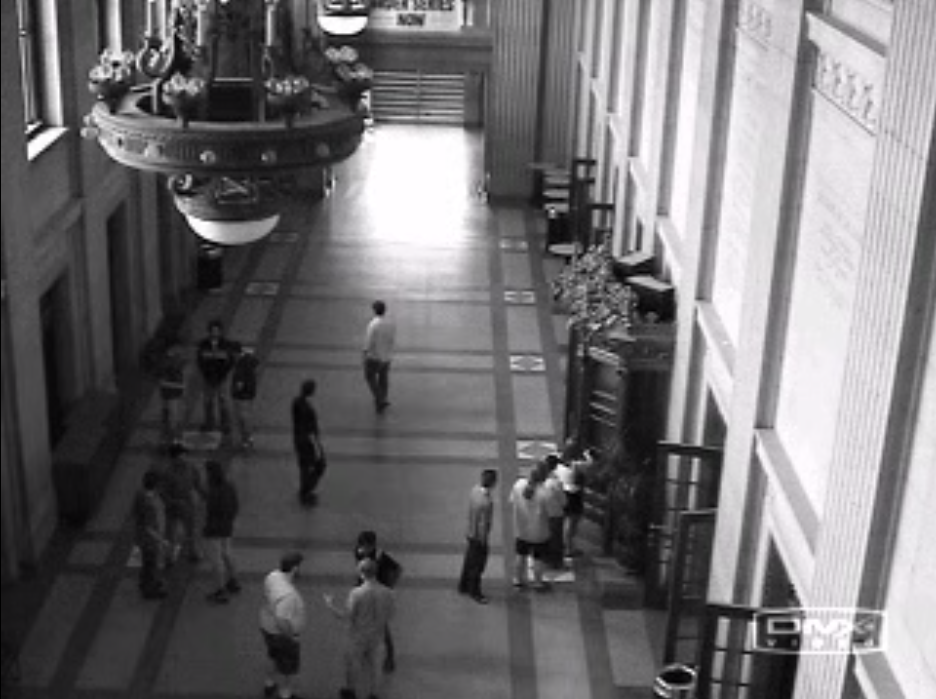
\includegraphics[width=0.8\linewidth]{images/umn_normal2.png}
         		\caption{Halls}
         		
         	\end{subfigure}\hfill%
         	\begin{subfigure}[t]{.3\textwidth}
         		\centering
         		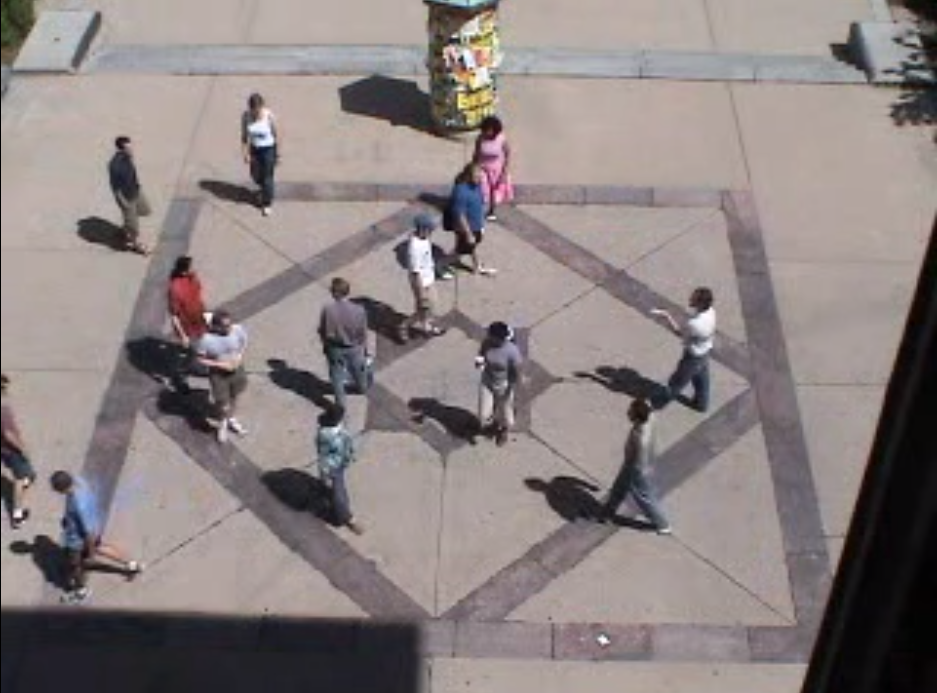
\includegraphics[width=0.8\linewidth]{images/umn_normal3.png}
         		\caption{Public pathways}
         		
         	\end{subfigure}
         	
         	\caption{\textbf{UMN-Crowd activity dataset} }
         	\label{umn_norm_ex}
         \end{figure}
         \item UMN crowd activity dataset:
         \begin{itemize}
         
         
   \item Total frames: 7719
   \item Anomalous frames: 1136
   \end{itemize}
   \item Demonstration datasets: KITTI and QMUL traffic junction dataset.
\end{itemize}
\end{frame}




\begin{frame}{Experiment}
\begin{table}[h]
	\centering
	
	
	\begin{tabular}{|l|l|}
		\hline
		Parameter                       & Value     \\ \hline
		Actual Frame Size               & 320 x 240 \\ \hline
		Dominant Orientation Image Size & 40 x 30   \\ \hline
		Frame Rate                      & 30 fps    \\ \hline
		No. of Frames / Prediction      & 30,20,10  \\ \hline
		Anomaly Detector Window Size    & 10 x 10   \\ \hline
		Noise Threshold                 & 0.05      \\ \hline
		Min. no. of Phase portrait changes                & 7    \\ \hline
	\end{tabular}
	\caption{Parameter Table}
	\label{table_para}
\end{table}
\end{frame}


\begin{frame}{Results}
   \begin{figure}[h!]
    	\begin{subfigure}[t]{0.3\textwidth}
    		%%%\vspace{0pt}
    		
    		\centering
    		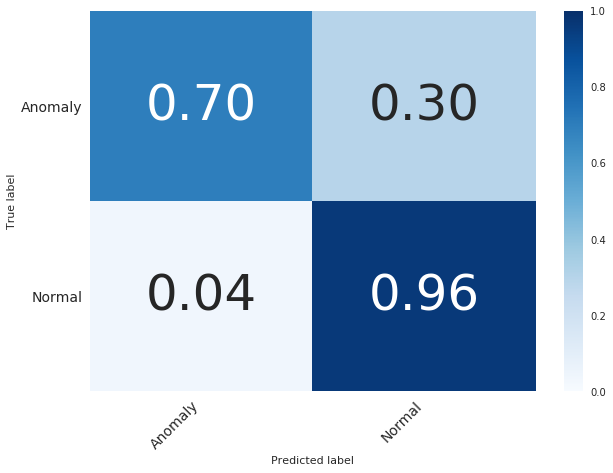
\includegraphics[width=0.65\linewidth]{images/30_cfmat.png}
    		
    		\caption{Prediction per 30 frames}
    	\end{subfigure}   
    	\begin{subfigure}[t]{.3\textwidth}
    		\centering
    		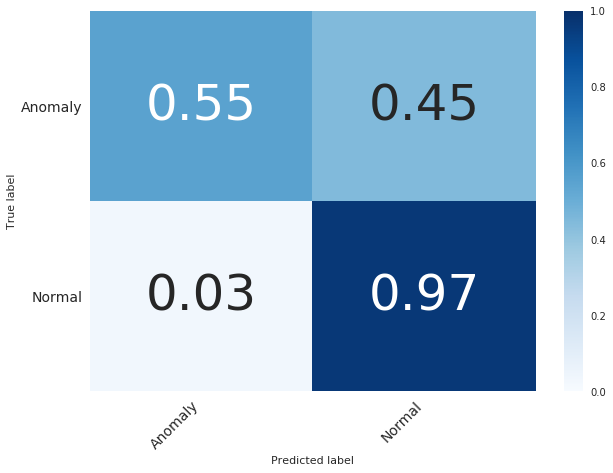
\includegraphics[width=0.65\linewidth]{images/20_cfmat.png}
    		\caption{Prediction per 20 frames }
    		
    	\end{subfigure}\hfill%
    	\begin{subfigure}[t]{.3\textwidth}
    		\centering
    		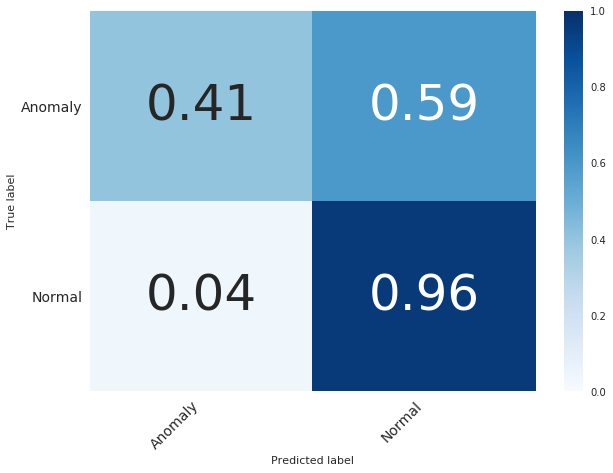
\includegraphics[width=0.65\linewidth]{images/10_cfmat.png}
    		\caption{Prediction per 10 frames}
    		
    	\end{subfigure}
    	
    	\caption{\textbf{Confusion Matrices:} The normalized confusion matrices for different prediction rates. Prediction per 30 frames works better than the other two. }
    	\label{fit_vary}
    \end{figure}
\begin{itemize}
\item The false negative values are high because some anomalous frames in between become the new normal in the anomalous sequence.
\item Performs significantly better with higher frames per prediction.
\item Algorithm does not capture well the sudden change in magnitude of flow values.
\end{itemize}
\end{frame}








\section{Contributions and future work}
\begin{frame}{Contributions and Future work}
\textbf{Contributions:}
\begin{itemize}
\item A context-independent motion anomaly detection algorithm.
\item A faster non-linear phase portrait classification algorithm by using evolution strategies.
\item A novel linear algorithm for phase portrait classification.
\item Evaluation of the performance of the detection algorithm on a real-time static camera scenario.
\item Demonstration of the generalizing capability with samples from dynamic camera scenarios.
\end{itemize}
\textbf{Future Work:}
\begin{itemize}

\item Rigorous testing with dynamic camera scenarios.
\item Testing with highly accurate optical flow estimators.
\item Integration with other methods for motion anomaly detection.
\end{itemize}

\end{frame}


\begin{frame}
  \frametitle{References}
  \printbibliography[title={References}]	
\end{frame}

\begin{frame}{Thank you!}
	\usebeamerfont{AAA}
	\begin{center}
		Questions?
	\end{center}
\end{frame}

\end{document}
